\documentclass[12pt]{article}
\usepackage{graphicx}
\usepackage{subcaption}
\usepackage{amsfonts}
\usepackage{amsmath}
\usepackage{fullpage}
\usepackage[utf8x]{inputenc}
\makeatletter
\usepackage{cite}
\usepackage{float}
\usepackage{hyperref}
\@namedef{opt@inputenc.sty}{utf8}
\makeatother
\usepackage{url}    
\usepackage{CJKutf8}
\usepackage{multirow}
\usepackage{array}
\newenvironment{conditions}
  {\par\vspace{\abovedisplayskip}\noindent\begin{tabular}{>{$}l<{$} @{${}={}$} l}}
  {\end{tabular}\par\vspace{\belowdisplayskip}}
\begin{document}
\title{
\begin{flushright}

\includegraphics[width=2.5cm]{logoUHi.jpg}\\
{\small
Data Analytics\\
Stiftung Universit{\"a}t Hildesheim\\
Marienburger Platz 22\\
31141 Hildesheim\\
Prof. Dr. Dr. Lars Schmidt-Thieme\\
}
\end{flushright}
\bigskip
\begin{center}
Thesis\\
Unsupervised Real-Time Time-Series Anomaly Detection\\
\end{center}
}
\author{Abdul Rehman Liaqat}
\date{271336, Liaqat@uni-hidesheim.de}
\maketitle

\newpage

\begin{abstract}
Anomaly detection is a crucial task for machine learning due to wide-spread usage and type. In particular, it is worth noting that most data arising in industrial setups are of a streaming nature, thus restricting the range of standard anomaly detection tools. This thesis will identify the potential approaches to learn the identification of abnormal behavior from large-scale streaming data. An empirical comparison of state-of-the-art methods will to be extended by a novel technical contribution. In this thesis, the focus is particularly on streaming time-series Anomaly Detection which changes in nature with time and novel contribution will especially try to target this dynamic nature of time-series.
\end{abstract}
\newpage
\tableofcontents
\newpage
\section{Introduction}
\subsection{Usage of streaming data}
With the increase in networking of objects, amount of data being generated is increasing. A big chunk of this data involves streaming data. Streaming data can be defined as data being generated continuously or with a continuous time interval. Since streaming data is generated continuously it is highly likely that it will keep on being generated forever. Best example of such streaming data is internet of things (IoT) sensors which almost all the time generate streaming data. Statistically, IoT data has grow from 4.4ZB (Zeta Bytes) to 44.4ZB with 50 billions devices. Also it is very likely that the data will change it's shape based upon external variables which are effecting the sensor or the data generating system itself. These devices include a small temperature sensor installed in a room to ECG data to satellite communication data. Even videos are kind of streaming data since they include data points (frames) separated by a constant interval. Data generated from human mounted sensors is also streaming data. Since the data being generated is continuous and infinite in nature, it is necessary to have techniques which are using data the same way. In other words, to make use of this data it is necessary to build system which are also running live and changing themselves online. Similarly, it is important to keep the system running as often times the components which are generating streaming data are at the core of the system and in case of failure of these components, there is a danger of whole system out of service. That is why it is necessary to find out any unusual behavior of the data generated by the component. Early detection of such unusual behavior can help avoid any catastrophic impact on the system. It can also alarm the system before the break down of any thing hence acting as predictive prevention. This kind of unusal behavior is called anomaly and such detection of such unusual behavior is called anomaly detection.\\
\break
An anomaly is defined as significantly different data point from other data points. The difference is dependent upon the at least two things. One is the data point being an outlier in general among all data points available. Second is that the data point value doens't make sense in the sequence data is being generated hence it is possible for new data point to be extremely different from all previous ones but still make sense to have in the sequence and vice versa. Detecting an anomaly helps in identifying abnormal behavior of a process with potentially useful information. In normal machine learning and data science projects, anomaly and outlier detection is an important step which will help clean the data and provide useful insights. \\
\break
Also as described in (reference name Software2), going forward software development especially machine learning based software development will be divided into two parts. One part is the preparation of the data and the second part is the design and optimization of algorithms. Both of these steps are used iteratively. Interestingly, as described in the (reference name Software2), more and more time is spent on accumulating, massaging and cleaning datasets. One major part of this process is outlier detection, anomaly detection and novelty detection. By detection of anomalies, it will become sufficiently easy for human expert to find the one data point in a heap of millions data points and then decide whether to remove that data or get more of the same data points.
\subsection{Usage of anomaly detection in streaming data}
As described above, anomaly detection is an important part of normal machine learning and data science projects. It is also very useful in streaming data systems. For example figure (\ref{machineTemperatureSystemFailure}) shows real-world temperature sensor data from an internal component of a large industrial machine. Anomalies are highlighted with red background. The second anomaly was a planned shutdown  hence there was an exceptional decrease in temperature. Last anomaly was a catastrophic system failure. Third anomaly just before the failure was a signal predicting the failure. If the anomlay detection system correctly detected the third anomaly system level failure could have been avoided hence saving a lot of time, money and resources.
\begin{figure}[H]
\centering
        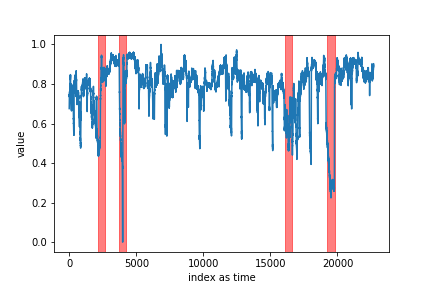
\includegraphics[width=\textwidth]{images/dataAnomalies/known/machine_temperature_system_failure.png}
    \caption{Machine Temperature System Failure}
    \label{machineTemperatureSystemFailure}
\end{figure}
Real-time data comes with special challenges and problems to solve for anomlay detection in streaming data. First constraint is the continuous arrival of data. 
We cannot have access to any future data. More specifically we will only have access to current time data as $x_t$ and previous data points as $x_{t-1},x_{t-2},x_{t-3},...$ and so on. This apply a constraint of finding the important of data in the past and update the model online. Also as the data stream is continuous it becomes evident to have the system doing online training and prediction. Thus the first contraint of an anomaly detection algorithm is that it should train and predict online.\\
\break
Secondly, the ending point of the stream is not known which means we should expect it to be an infinite amount of data beign received continuously. Also most of the time to identify an anomaly help of a domain expert is needed. For this reason and possibly continuous changing state of the data (as described as concept drift up next) the model should be updated with latest labels. Consequently, it becomes impossible to have access to enough labeled data which is kept updated all the time. That is why an unsupervised anomaly detection system is prefered which will always update itself according to system change and we will not need to setup some manual training steps.\\
\break
Before moving on, there are some unique concepts related to uni-variate time series which will be helpful in the understanding of the research problem. Starting with stationary and non-stationary time series. A stationary time series is the one whose statistical properties are constant over time. These statistical properties include mean, variance and auto-correlation of the time series. Similarly with the change in one or more of these statistical properties, non-stationary time series comes into being. These non-stationary time series are also named as Concept drift. Concept drift is a terminology related to time series data specifically which is why we will be using the term Concept drift instead of non-stationary time series in future. There is also an intuitive meaning behind the name of Concept drift.\\
\break
Considering that there is an underlying probability distribution in every time series and this underlying distribution is named Concept of time series such as
\begin{equation}
Concept =  P_t(X)
\end{equation} 
The the concept drift occurs between two times t and u when the distribution or concept changes as
\begin{equation}
    P_t(X) \neq P_u(X)
\end{equation}
And the new data points are generated from the second distribution $p_u(X)$ onward rather then the original $P_t(X)$ for a length of time $T$. This time $T$ is decided by the domain knowledge and frequency of data points.
As in real life systems it is highly likely that there will be a change in the concept of the time-series hence happening of concept drift is very likely and possible. For example, there will be a concept drift in the time-series output of a heat sensor measuring the temperature of a motor of exhaust fan and the motor of the fan is changed. Thus it is necessary for our system to first recognize the concept drift. If there exists a concept drift then the model should adapt itself swiftly to avoid false positives. Similarly if there is not a concept drift then the model should not give much learning weight to these readings. Thus the model adaption according to presence of concept drift is necessary.\\
\break
Time series data is the output of a streaming data from multiple devices which makes it close to impossible to label it specially for anomalies. Also due to concept drift a regular labeling needed. Since it is very difficult to label streaming time series data to detect anomalies it makes sense to do it in an unsupervised fashion. With unsupervised anomaly detection we don't need any previous labeled data and the system developed will be very generic.
An anomaly is defined as a data point $X_t$ or set of data points $X_{t-l:t}$ for which either of following is true
$\gg \ll$ Example of each anomaly
\begin{enumerate}
    \item Probability of point $X_t$ belonging to a probability distribution $\phi$ is very less then the probability of previous data points $X_n$ where $n \leq t-1$. In other words:\\
    \begin{equation}
        P(X_t) \in \phi  \ll P(X_n) \in \phi 
    \end{equation}
    This type of anomaly is called point anomaly. Here $\phi$ is the probability distribution generating all the data points.
    \item Probability of points $X_{t-l:t}$ belonging to a probability distribution $\phi$ is very less then the probability of $X_{n-l:n}$ where $n \leq t-1$. In other words: \\
    \begin{equation}
        P(X_{t-l:t}) \in \phi  \ll P(X_{n-l:n}) \in \phi         
    \end{equation}
        This type of anomaly is called collective anomaly.
    \item Probability of point $X_t$ belonging to a probability distribution $\phi$ is almost same as the probability of previous data points $X_n$ where $n \leq t-1$ but the probability of point $X_t$ belonging to a probability distribution $\theta$ is very less than the probability of point $X_p$ belonging to $\theta$. Here In other words:\\
    \begin{equation}
        P(X_t) \in \phi  \approx P(X_n) \in \phi 
    \end{equation}
    \begin{equation}
        P(X_t) \in \theta  \ll P(X_n) \in \theta 
    \end{equation}
    Here $\theta$ and  $X_p$ are probability distribution and data points. $theta$ is a distribution defined to a set of local points $X_p$ where $p \leq t$ and $p$ is a set of indices. 
    This type of anomaly is called Contextual anomaly. 
\end{enumerate}
As defined above, in many cases there is a system change which causes a permanent change in the probability distribution being generated by the data. As example is in figure \ref{awsCpuUtilizationConceptDrift}, where software updates and configuration changed can change the behavior of the system forever. Now the system must adapt to detect anomalies according to the new type of data. To do that the model must first recognize that if it is a concept drift and then change itself accordingly that too in an unsupervised and automated way.
\begin{figure}[H]
\centering
        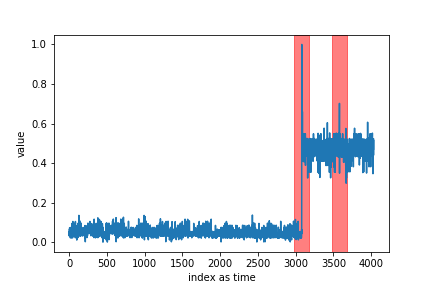
\includegraphics[width=\textwidth]{images/dataAnomalies/aws/rds_cpu_utilization_cc0c53.png}
    \caption{AWS CPU Utilization Concept Drift}
    \label{awsCpuUtilizationConceptDrift}
\end{figure}
In streaming applications it is also very useful to detect the anomaly as early as possible. For example in the streaming data of cardiac patient's heart, earlier detection can help in taking emergency measures to stop the onset of heart attack. Obviously detecting them a little earlier is way better tham later. This early detection acts as an alarm and will really fulfill the purpose of alarm when enough time is remaining to take action to avoid catastrophic failure. Of course, having this early detection property of an algorithm comes with drawbacks. One drawback is that extra senstivity of the algorithm, which can cause many false alarms. Therefore there is a trade-off between false alarms and  true positives. Using the above properties of the anomaly detection algorithm we can define the characteristics of an unsupervised real-time anomaly detection algorithma as:
\begin{enumerate}
\item Predictions must be made online which means that the algorithm must identify state $x_t$ as normal or anomalous before receiving the next data point $x_{t+1}$
\item The algorithm msut learn continuously without a requirement to store the entire stream. 
\item The algorithm must run in an unsupervised, automated fashion. In other words the algorithm should not be fed any labeled data or shouldn't have any manual parameter changing.
\item Algorithms must adapt to dynamic environments and concept drift, as the underlying probability distributions often change.
\item Algorihtms should make anomaly detections as early as possible.
\item Algorithms should minimize false positives and false negatives.
\end{enumerate}
Of course, it is difficult to fulfill all the requirement. Still the best detection algorithm will try to maximize the completion of all above. Secondly based upon the requirement of the system few requriements can also be relaxed.
Concluding, with the requriements given above it becomes obvious that many current anomaly detection algorithms do not fulfill them.\\
\break
Now to detect all the type of anomalies described above it is necessary to estimate the underlying probability distributions responsible for generating the stream. In general there are following few steps in an Anomaly detection framework as described in figure \ref{generalAnomalyDetectionFrameWork}.\\
\break
First step is to pre-process the input data. We use min-max normalization to make sure that all input values are limited between $0$ and $1$. Min-max normalization can be defined as
\begin{equation}
    z = \frac{x - min(x)}{max(x) - min(x)}
    \label{minMaxNormalization}
\end{equation}
Second step is to estimate the underlying probability distribution by building a model. This model can be used to model the streaming time series. \\
\break
Next step would be to score the incoming data point. At this moment we will use the previously estimated probability distribution and types of anomalies defined above to score the incoming data point. \\
\break
Afterwards the score is passed through a post-processing step. In this step possibly normalization and probabilistic likelihood estimation is applied on top of the previously calculated anomaly score. In other words previously calculated anomaly score is transformed between the range of $0$ and $1$. \\
\break
After post-processing, we can use this score to actually rank each incoming data point among previously existing data points. To label each data point as anomaly or not anomaly a thresholding procedure is necessary. Depending upon the type of post-processing extreme cases are considered as anomalies.
\begin{figure}[H]
\centering
        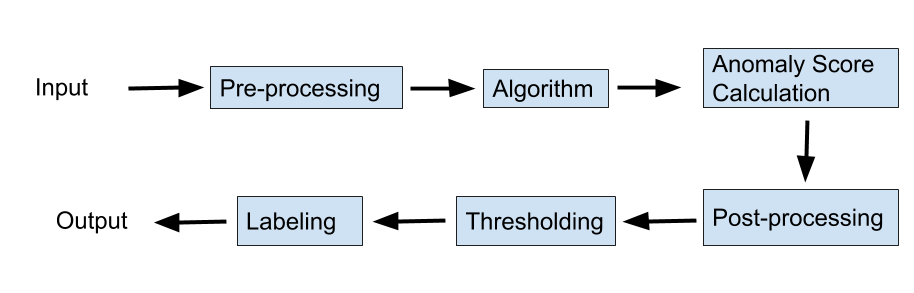
\includegraphics[width=\textwidth]{images/generalAnomalyDetectionFrameWork.png}
    \caption{General Anomaly Detection Framework}
    \label{generalAnomalyDetectionFrameWork}
\end{figure}
Thus there are many possible points of innovation in the anomaly detection framework based upon the type of problem we are facing. A quick brief of these likely innovations are following:
\begin{enumerate}
    \item First possible innovation is done at the pre-processing step. Here it is very helpful to normalize the input data and constrain it between $0$ and $1$. The benefits of normalization show up while calculating anomaly score as anomaly score will be then close to the range of $0$ and $1$. Another very important point is  
    \item Second and a major problem to solve is the algorithm that will estimate the probability distribution of streaming data. This algorithm should have at least following properties:
    \begin{itemize}
    	\item The algorithm should have the capability to differentiate the concept drift with actual anomalies and adapt itself accordingly.
    	\item The algorithm cannot look ahead in the future values. In other words the algorithm will work on real-time streaming data and will only be dependent upon current and past values.
    	\item It should be able to train itself ideally, before the arrival of next data point. This condition will make the algorithm fast and online.
    \end{itemize}
	\item Another possible innovation area is the values the algorithm is trained for. The algorithm can be an autoencoder based and be used to reconstruct a window of current and past values hence predicting a sequence which will then be compared with original values. The distance between the predicted sequence of reconstruction and actual values will be used as anomaly score then. Otherwise using a sub-sequence, one can predict another sub-sequence which is few time step ahead of the input sequence. The autoencoder learns how to reconstruct the current sequence and predictive learns how to predict the future values. 
	\item Now that we have an anomaly score, next step is to apply some post-processing on top of this score. There are two possible variations used. First variation is moving min-max normalization. With this kind of normalization current point is normalized by using the minimum and maximum values of the data obtained so far. Seoncd type of post-processing is probability of values of a current small window from the previous values.
\end{enumerate}
\newpage
\section{Related Work and State of the art}
Here we will slowly build up to the techniques which are used in sate-of-the-
art anomaly detection methods. Anomaly detection in time-series has been heavily studied since a long time. Many anomaly detection approaches exist as supervised, semi-supervised and unsupervised approach. Although most of them rarely process data online. For example the robust principle component analysis (RPCA) developed by Netflix requires complete dataset to to find out anomaly. Similarly EGADS developed by yahoo need access to whole data. A simpler techniques used is symbolic aggregate approximation or SAX which requires the decomposition of time series into symbols before treating them. \\
\break

Anomaly detection in time-series is a heavily studied area
of data science and machine learning, dating back to [5] . Many
anomaly detection approaches exist, both supervised (e.g. support
vector machines and decision trees [6] ) and unsupervised (e.g.
clustering), yet the vast majority of anomaly detection methods
are for processing data in batches, and unsuitable for real-time
streaming applications. Examples from industry include Netflix’s
robust principle component analysis (RPCA) method [7] and Ya-
hoo’s EGADS [8] both of which require analyzing the full dataset.
Likewise, Symbolic Aggregate Approximation (SAX) [9] involves
decomposing the full time series to generate symbols prior to
anomaly detection. Other recent techniques include [10,11] . Al-
though these techniques may work well in certain situations, they
are traditional batch methods, and the focus of this paper is on
methods for online anomaly detection. For reviews of anomaly de-
tection in general we recommend [1,6,12,13] . For prior work on
data stream mining and concept drift in general see [3,14–17] .
Some anomaly detection algorithms are partially online. They
either have an initial phase of offline learning, or rely on look-
ahead to flag previously-seen anomalous data. Most clustering-
based approaches fall under the umbrella of such algorithms.
Some examples include Distributed Matching-based Grouping Al-
gorithm (DMGA) [18] , Online Novelty and Drift Detection Algo-
rithm (OLINDDA) [19] , and MultI-class learNing Algorithm for data
Streams (MINAS) [20] . Another example is self-adaptive and dy-
namic k-means [21] that uses training data to learn weights prior
to anomaly detection. Kernel-based recursive least squares (KRLS)
proposed in [22] also violates the principle of no look-ahead as it. Some anomaly detection algorithms are partially online. They
either have an initial phase of offline learning, or rely on look-
ahead to flag previously-seen anomalous data. Most clustering-
based approaches fall under the umbrella of such algorithms.
Some examples include Distributed Matching-based Grouping Al-
gorithm (DMGA) [18] , Online Novelty and Drift Detection Algo-
rithm (OLINDDA) [19] , and MultI-class learNing Algorithm for data
Streams (MINAS) [20] . Another example is self-adaptive and dy-
namic k-means [21] that uses training data to learn weights prior
to anomaly detection. Kernel-based recursive least squares (KRLS)
proposed in [22] also violates the principle of no look-ahead as it resolves temporarily flagged data instances a few time steps later
to decide if they were anomalous. However, some kernel methods,
such as EXPoSE [23] , adhere to our criteria of real-time anomaly
detection (see evaluation section below).
For streaming anomaly detection, the majority of methods
used in practice are statistical techniques that are computation-
ally lightweight. These techniques include sliding thresholds, out-
lier tests such as extreme studentized deviate (ESD, also known
as Grubbs’) and k-sigma (e.g., [24,25] ), changepoint detection [26] ,
statistical hypotheses testing, and exponential smoothing such as
Holt–Winters [27] . Typicality and eccentricity analysis [28,29] is an
efficient technique that requires no user-defined parameters. Most
of these techniques focus on spatial anomalies, limiting their use-
fulness in applications with temporal dependencies.
More advanced time-series modeling and forecasting models
are capable of detecting temporal anomalies in complex scenar-
ios. ARIMA is a general purpose technique for modeling temporal
data with seasonality [30] . It is effective at detecting anomalies in
data with regular daily or weekly patterns. Extensions of ARIMA
enable the automatic determination of seasonality [31] for certain
applications. A more recent example capable of handling temporal
anomalies is the technique in [32] based on relative entropy.
Model-based approaches have been developed for specific use
cases, but require explicit domain knowledge and are not gener-
alizable. Domain-specific examples include anomaly detection in
aircraft engine measurements [33] , cloud datacenter temperatures
[34] , and ATM fraud detection [35] . Kalman filtering is a com-
mon technique, but the parameter tuning often requires domain
knowledge and choosing specific residual error models [12,36–38] .
Model-based approaches are often computationally efficient but
their lack of generalizability limits their applicability to general
streaming applications. There are a number of other restrictions that can make meth-
ods unsuitable for real-time streaming anomaly detection, such as
computational constraints that impede scalability. An example is
Lytics Anomalyzer [39] , which runs in O ( n 2 ), limiting its useful-
ness in practice where streams are arbitrarily long. Dimensionality
is another factor that can make some methods restrictive. For in-
stance online variants of principle component analysis (PCA) such
as osPCA [40] or window-based PCA [41] can only work with high-
dimensional, multivariate data streams that can be projected onto
a low dimensional space. Techniques that require data labels, such
as supervised classification-based methods [42] , are typically un-
suitable for real-time anomaly detection and continuous learning.
Additional techniques for general purpose anomaly detection
on streaming data include [9,43,44] . Twitter has an open-source
method based on Seasonal Hybrid ESD [45] . Skyline is another
popular open-source project, which uses an ensemble of statisti-
cal techniques for detecting anomalies in streaming data [24] . We
include comparisons to both of these methods in our Results sec-
tion.
\subsection{Unsupervised Anomaly Detection}
In unsupervised anomaly detection, there are five differet type of algorithms used. First type is nearest-neighbor based. These methods 
\begin{enumerate}
	\item Time series intro. Prediction and classification.
	\item Unsupervised methods on time series 
	\item Anomaly detection
	\item Time series Anomaly detection
	\item Unsupervised Time series Anomaly detection
	\item General components latest anomaly detection methods and explanation of each
	\item HTM based anomaly detection paper review. Problems or way it does it
	\item paper 2
	\item paper 3
	\item general review, problems, bottlenecks and trend
\end{enumerate}
\newpage
\section{Proposed method}
\subsection{General anomaly score based architecture and detailed explanation}
\begin{figure}[H]
\centering
        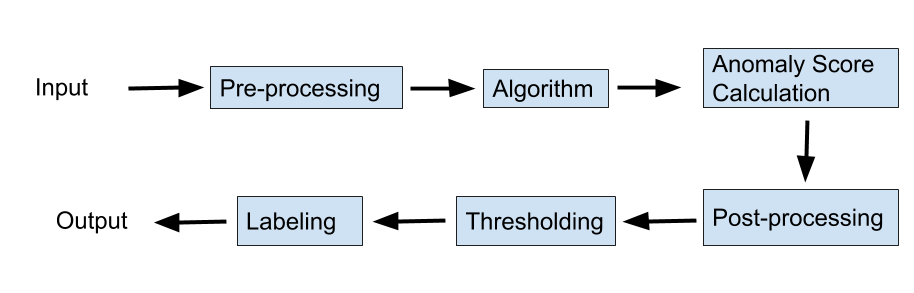
\includegraphics[width=\textwidth]{images/generalAnomalyDetectionFrameWork.png}
    \caption{General Anomaly Detection Framework}
    \label{generalAnomalyDetectionFrameWork}
\end{figure}
Considering figure ~\ref{generalAnomalyDetectionFrameWork}, each algorithm will be using  
all parts with few variations and a cusotmized algorithm part.\\
\break
Pre-processing is playing crucial role in the generalization of the algorithms. There are two different kind of normalization techniques tested. First kind is global normalization
Proposed method can be divided in multiple parts. First part would be the implementation of baselines using latest deep learning architectural components. The main components of our anomaly detection framework are as following:
\begin{itemize}
\item In the pre-processing part, each time-series is normalized using equation \ref{minMaxNormalization}. Here we assume that we already know the possible minimum and maximum values of the data which is generally true in most cases. All the dataasets are normalized before feeding into the algorithm.
\item In the algorithm part, we use different kind of algorihtms with few things in common. For all kind of algorithms the input values are sequence of length $W$ and output values are also a sequence whose size is tested from $1$ to $5$. Another important thing to remember is that the output is different for autoencodre based architectures and multistep prediction architectures. More details are given below.
\item We take the simple mean squared distance as anomaly score. So at each time step, we take the difference between the output sequence and the actual real sequence using mean squared distance. The same is also used for training of each algorithm. After doing a forward pass prediction and calculating the anomaly score using mean squared distance, we use the anomaly score to back-propagate the error using one iteration.
\item Next post-processing step is important as literature shows that this step makes a significant difference in the improving the score of an anomaly detector. There are two different kind of post-processing techniques used. First technique is the usage of anomaly likelihood as described equation.
The anomaly likelihood is a probabilistic metric defining how anomalous the current state is based on the prediction history.To compute the anomaly likeli-
hood we maintain a window of the last W error values. We model
the distribution as a rolling normal distribution where the sample
mean $\mu_t$ and variance $\sigma^2_t$, are continuously updated from previ-
ous error values as follows:
\begin{equation}
\mu_t = \frac{\sum_{i=0}^{i=W-1} S_{t-i}}{W}
\end{equation}
\begin{equation}
\sigma^2_t=\frac{\sum_{i=0}^{i=W-1} (S_{t-i}-\mu_t)^2}{W-1}
\end{equation}

We then compute a recent short term average of prediction
errors, and apply a threshold to the Gaussian tail probability
to decide whether or not to declare an anomaly. 3
We define the anomaly likelihood as the complement of the tail
probability:
\begin{equation}
L_t = 1-Q (\frac{\tilde{\mu_t}-\mu_t}{\sigma_t})
\end{equation}
and here $\tilde{\mu_t}$ is defined as:
\begin{equation}
\tilde{\mu_t} = \frac{\sum_{i=0}^{i=w-1}S_{t-i}}{w}
\end{equation}
Here $w \ll W$. We use $w$ for short term moving average and $W$ for long term moving average. This will give us a probability likelihood of a data point being an anomaly. Next step is to threshold the anomlay by setting up a threshold which is defined by user and is a hyperparameter. The threshold is set to $1-\epsilon^{-5	}$
\item Second method is moving mix-max normalization, which is rather simple but quite effective. We take the maximum and minimum value of the past and current data at a given point in time $T$ and use it to normalize the incoming anomaly score value. If the new anomaly score value is greater than the past maximum value then the maximum value is updated. Similarly if the new anomaly score value is less than the past minimum value then the minimum value is updated. In the beginning of training, ususally convergence loss is higher and it does not make sense to compare it with the values calculated later on that is why first $N$ value of the anomaly score are skipped before we start considering the maximum and minimum value. The value $N$ is usually set around $100$.
\end{itemize}
We use these components to develop two different kind of detectors.\\
\break
One detector is based upon prediction of a next data point. Let $T_{(t-L-1):(t-1)}$ is the small window taken from time series. The starting point is $t-L-1$ where $L$ is the window size and last data point is taken from $t-1$ which is the data point at previous time step. This data window is used to predict the time series value at time $t$. To predict at time $t$ various different kind of functions as baselines using latest architectural components are designed. Generally the output of such a function would be
\begin{equation}
f(T_{(t-L-1):(t-1)}) = \hat{f}(t)
\end{equation} 
Thus the function $f$ in prediction based models map data points as: $f: L \mapsto 1$ where $L$ is the window size and output is the prediction of value at current time. For optimization of function $f$, the difference between time series value at current time step and predicted value at current time is taken. More specifically the objective function will be
\begin{equation}
min |\hat{f}(t) - f(t)|
\end{equation}
That is to minimize the difference between time series value at time $t$ and predicted time series value at time $t$ using time series value from $T_{(t-L-1):(t-1)}$.
\subsection{Autoencoder based architecture}
An autoencoder is a network which is trained to copy its input to its output, with the typical purpose of dimension reduction - the process of reducing the number of random variables under consideration. It features an encoder function to create a hidden layer (or multiple layers) which contains a code to describe the input. There is then a decoder which creates a reconstruction of the input from the hidden layer. An autoencoder can then become useful by having a hidden layer smaller than the input layer, forcing it to create a compressed representation of the data in the hidden layer by learning correlations in the data. This compressed representation is actually summarized version of input. This way for the anomaly input values, summarized version will not output very similar output and hence ending up creating big reconstruction loss.
The backpropagation will try to  $h_{W,b}(x) \approx x$ , so as to minimise the mean square difference:
\begin{equation}
L(x,y) = \sum(x-h_{W,b}(x))^2
\end{equation}
Similarly for time series let $X_t$ be the input value of the streaming data at time $t$ then the input of autoencoder based architecture will be $X_{t-w:t}$ and output will be $Y_{t-w:t}$ as $Y$ is the predicted reconstruction of the input. 
\begin{equation}
Y_{t-w:t} = h(X_{t-w:t})
\end{equation}
The reconstruction loss is defined as:
\begin{equation}
L(x,y) = \frac{1}{w}\sum(Y_{t-w:t}-X_{t-w:t})^2
\end{equation}
$\gg \ll$ picture of an autoencoder
\subsection{Multistep-Ahead based architecture}
$\gg \ll$ picture of an multi-step based architecture
Second type of architecture used is multi-step prediction architecture. In this type of architecutre 
For time series let $X_t$ be the input value of the streaming data at time $t$ then the input of multistep prediction based architecture will be $X_{t-w-l:t-l}$ and output will be $Y_{t-l:t}$ as $Y$ is the prediction of the input. 
More specifically
\begin{equation}
Y_{t-l:t} = h(X_{t-w-l:t-l})
\end{equation}
and the prediction loss will be defined as:
\begin{equation}
L(x,y) = \frac{1}{l}\sum(Y_{t-l:t}-h(X_{t-w-l:t-l}))^2
\end{equation}

Above two are the basic outputs which are repeated with following different architectures.
\subsection{Fully connected architecture}
\begin{figure}[H]
\centering
        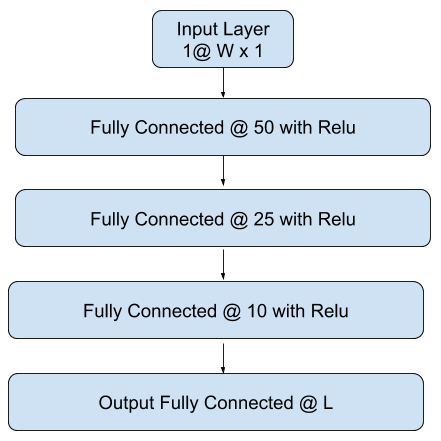
\includegraphics[width=\textwidth]{images/architecture/NnMultistepAheadPrediction.png}
    \caption{Fully connected autoencoder}
    \label{generalAnomalyDetectionFrameWork}
\end{figure}
\subsection{Fully connected prediction architecture}
\begin{figure}[H]
\centering
        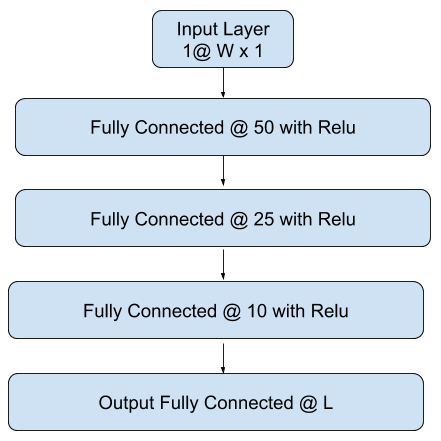
\includegraphics[width=\textwidth]{images/architecture/NnMultistepAheadPrediction.png}
    \caption{Fully Connected Multistep Prediction Architecture}
    \label{generalAnomalyDetectionFrameWork}
\end{figure}
\subsection{Fully connected autoencoder architecture}
\subsection{Convolution based prediction architecture}
\begin{figure}[H]
\centering
        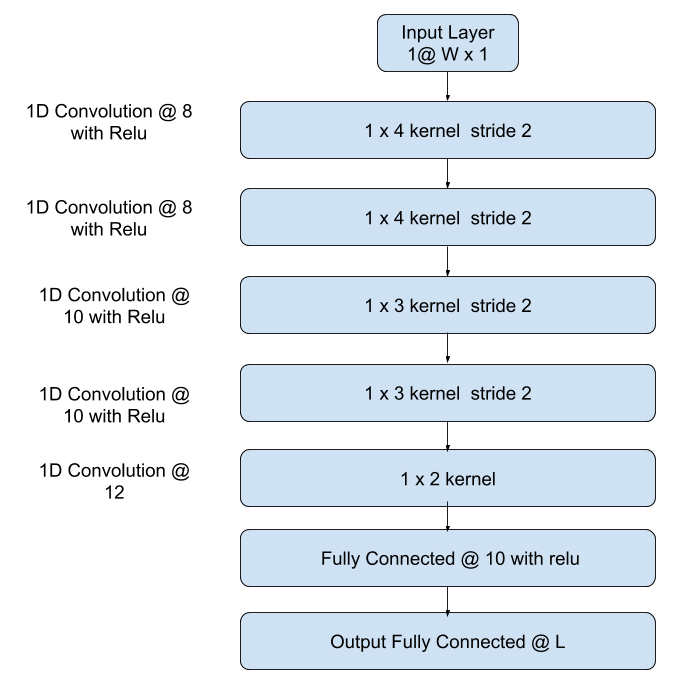
\includegraphics[width=\textwidth]{images/architecture/CnnMultistepPrediction.png}
    \caption{Convolutional Network based Prediction Network}
    \label{generalAnomalyDetectionFrameWork}
\end{figure}
\subsection{LSTM based prediction architecture}
\begin{figure}[H]
\centering
        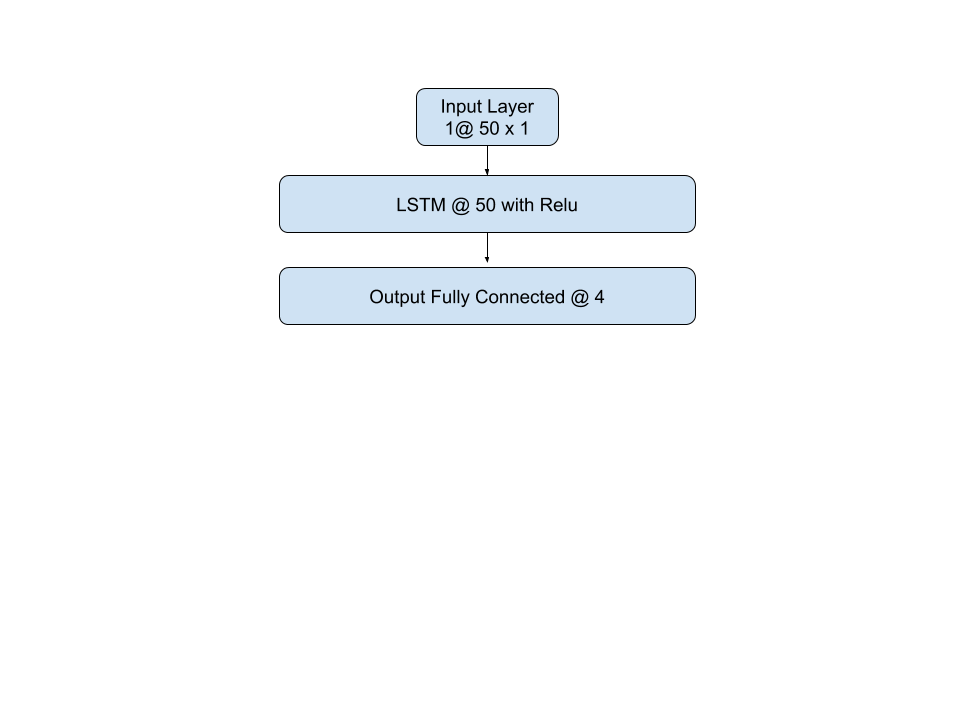
\includegraphics[width=\textwidth]{images/architecture/LstmMultistepaheadPrediction.png}
    \caption{LSTM based Prediction Network}
    \label{generalAnomalyDetectionFrameWork}
\end{figure}
\subsection{LSTM based autoencoder based architecture}
\subsection{Recency concept}
\subsection{Post-processing}
\subsection{Thresholding}
\subsection{Parameterinzing the anomaly score}
\newpage 
\section{Empirical Formulation and Experiments}
\subsection{Dataset}
To experiment with proposed method and campare them with state-of-the-art results Numenta Anomaly Benchmark (NAB) was used. Numenta is a benchmark specifically designed for online time series anomaly detection.\\
\break
Using NAB provides with many benefits. First is a benchmark dataset which $58$ various univariate time series, each with timestamp as index and value. Length of each time series ranges from $1000$ to $22000$ data points. These $58$ time series are from six different categories. These categories include artificially generated time series, times series gathered from advertisement industry related data such as click through rate (CTR), AWS usage metrics, server traffic data, tweets volume time series and known cause anomaly which has the a solid reason for the labeled anomaly.\\
\break
The diversity of these categories provide the second benefit. With the diversity almost all type of anomalies are covered hence each algorithm can be tested against each type. Artificial datasets further contains time series with anomalies and without anomalies. Datasets without anomalies contain only normal patterns and no anomaly thus any predicted anomaly will be a false positive here. 
\begin{figure}[H]
  \begin{subfigure}[t]{.5\textwidth}
    \centering
    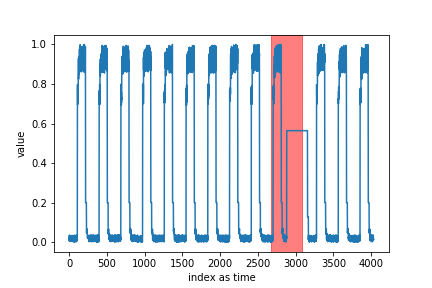
\includegraphics[width=\linewidth]{images/dataAnomalies/artificial/art_daily_flatmiddle.png}
    \caption{Artificial with sudden flat-middle}
  \end{subfigure}
  \hfill
  \begin{subfigure}[t]{.5\textwidth}
    \centering
    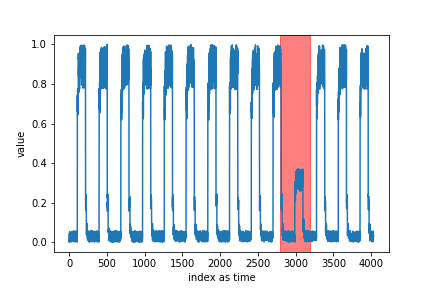
\includegraphics[width=\linewidth]{images/dataAnomalies/artificial/art_daily_jumpsdown.png}
    \caption{Artificial with sudden jumps-down}
  \end{subfigure}

  \medskip

  \begin{subfigure}[t]{.5\textwidth}
    \centering
    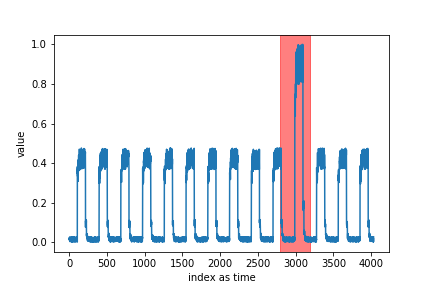
\includegraphics[width=\linewidth]{images/dataAnomalies/artificial/art_daily_jumpsup.png}
    \caption{Artificial with sudden jumps-up}
  \end{subfigure}
  \hfill
  \begin{subfigure}[t]{.5	\textwidth}
    \centering
    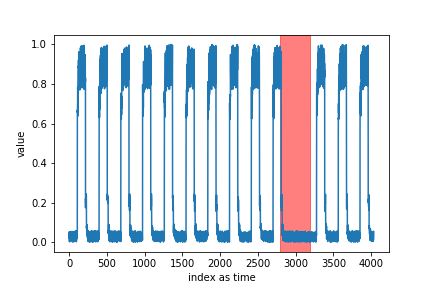
\includegraphics[width=\linewidth]{images/dataAnomalies/artificial/art_daily_nojump.png}
    \caption{Artificial with sudden flat}
  \end{subfigure}
  \caption{Examples of artifical anomaly data set}
  \label{artificialDataPlots}
\end{figure}

Many datasets contains concept drift. These datasets are mostly real life ones. Example of these are following:

\begin{figure}[H]
  \begin{subfigure}[t]{.5\textwidth}
    \centering
    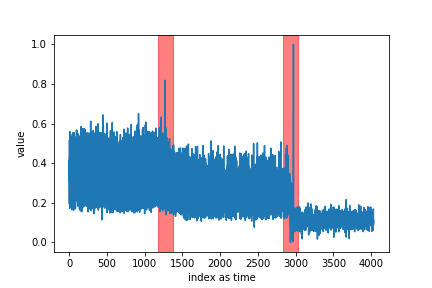
\includegraphics[width=\linewidth]{images/dataAnomalies/aws/ec2_cpu_utilization_5f5533.png}
    \caption{Artificial with sudden flat-middle}
  \end{subfigure}
  \hfill
  \begin{subfigure}[t]{.5\textwidth}
    \centering
    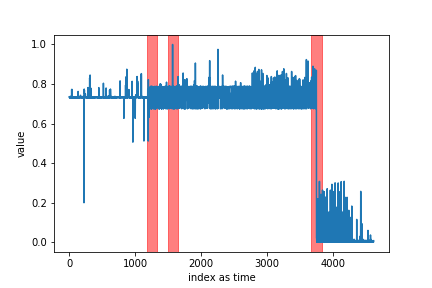
\includegraphics[width=\linewidth]{images/dataAnomalies/aws/grok_asg_anomaly.png}
    \caption{Artificial with sudden jumps-down}
  \end{subfigure}

  \medskip

  \begin{subfigure}[t]{.5\textwidth}
    \centering
    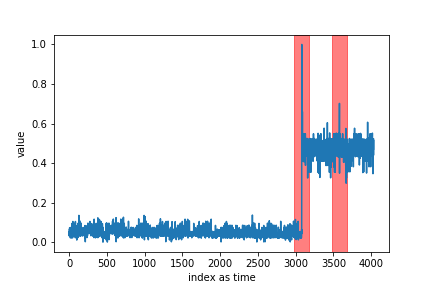
\includegraphics[width=\linewidth]{images/dataAnomalies/aws/rds_cpu_utilization_cc0c53.png}
    \caption{Artificial with sudden jumps-up}
  \end{subfigure}
  \hfill
  \begin{subfigure}[t]{.5	\textwidth}
    \centering
    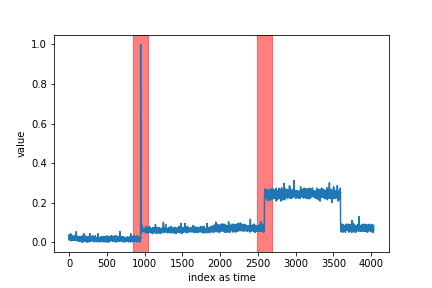
\includegraphics[width=\linewidth]{images/dataAnomalies/aws/rds_cpu_utilization_e47b3b.png}
    \caption{Artificial with sudden flat}
  \end{subfigure}
  \caption{Examples of Concept drift in AWS data sets}
  \label{AwsConceptDrift}
\end{figure}

Similarly almost all kind of anomalies exist in the dataset. For example for point anomaly we can see that in following.

\begin{figure}[H]
  \begin{subfigure}[t]{.5\textwidth}
    \centering
    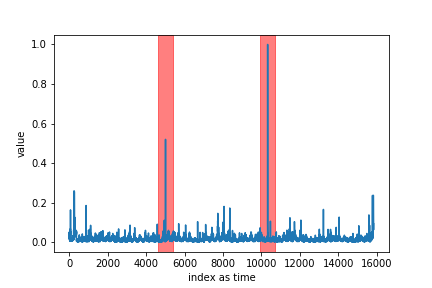
\includegraphics[width=\linewidth]{images/dataAnomalies/twitter/Twitter_volume_FB.png}
  \end{subfigure}
  \hfill
  \begin{subfigure}[t]{.5\textwidth}
    \centering
    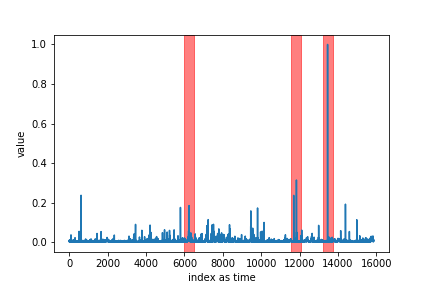
\includegraphics[width=\linewidth]{images/dataAnomalies/twitter/Twitter_volume_KO.png}
  \end{subfigure}

  \medskip

  \begin{subfigure}[t]{.5\textwidth}
    \centering
    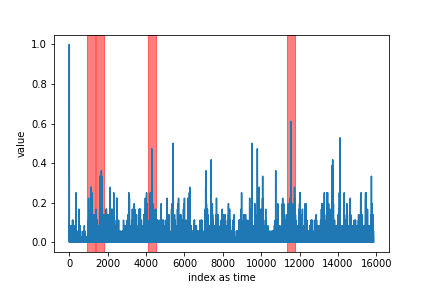
\includegraphics[width=\linewidth]{images/dataAnomalies/twitter/Twitter_volume_PFE.png}
  \end{subfigure}
  \hfill
  \begin{subfigure}[t]{.5	\textwidth}
    \centering
    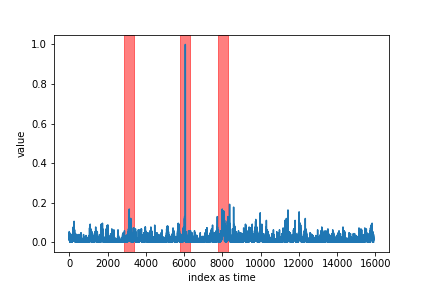
\includegraphics[width=\linewidth]{images/dataAnomalies/twitter/Twitter_volume_CRM.png}
  \end{subfigure}
  \caption{Examples of point anomalies from twitter volume dataset}
  \label{AwsConceptDrift}
\end{figure}

Another important benefit is the availability of labeled data. Other then the seven time series for which we know the existance of anomaly, others were labeled using following process.
\begin{enumerate}
\item A number of human labelers have labeled the benchmark dataset. Each individual labeler read through the published labeling guidelines, and then looked through the individual data files in the benchmark dataset, using data visualization methods. They recorded the timestamps at which anomalies appeared to start. The collection of these labels for all the data
files makeup the raw labels files, one for each labeler and data batch.
\item Each raw label file is a dictionary of key-value pairs, where the dataset
name identifies a list of labeled anomaly timestamps. Across these files,
the timestamps are compared to identify the ground truth anomalies,
yielding one ground truth label file. To determine the true anomalies, a
custom “bucket-merge” algorithm is used:
\begin{enumerate}
\item For each given data file (i.e. the key), the start timestamps from all
the raw labels are collected into buckets with other start timestamps
within a certain range. That is, timestamps within a narrow range of
one another are bucketed together because they (very likely)
identify the same anomaly. Differences in anomaly start times
amongst labelers can be attributed to human error. The size of the
time range is set as 1/10 the size of an anomaly window (defined in
step 3 below), both preceding and following the given timestamp.
The rationale is straightforward: following the underlying
assumption anomalies are rare, if multiple anomaly labels fall within
the same window, they identify the same sequence of anomalous
data.
\item If a given bucket contains more timestamps (raw labels) than the
agreement threshold, it is classified as a true anomaly. The
standard threshold is 0.50, so a bucket must contain timestamps
from 50\% or more of the labelers in order to become a true
anomaly label .
\item Each true anomaly bucket is then merged into a single timestamp
based on frequency. That is, the timestamp which appears most
often within a bucket is chosen to represent the entire bucket. Ties
are determined by which timestamp occurs first. The resulting
timestamps are the ground truth labels marking the start of the true
anomalies.
\end{enumerate}
\item The combined labels are then converted into anomaly windows, indicated
by a beginning and ending timestamp. The motivation behind anomaly
windows is twofold. First, anomalous data often occurs over time, rather
than at a single point, and thus defining anomaly windows improves the
NAB scoring efficacy. Second, anomaly windows allow the DUT to not be
penalized during scoring if the DUT anomaly detections are slightly before
or after the ground truth. We want these windows to be large enough to
allow early detection of anomalies, but not so large as to artificially boost
the score of inaccurate detectors. That is, the windows give the benefit of
the doubt to the detector, but not so much that false positives would count
as true positives. The anomaly windows are calculated using the following
algorithm:
\begin{enumerate}
\item The total amount of window length in a single data file was chosen
to be 10\% of the data file length. For instance, if a data file contains
4000 data points, then the total amount of relaxation shared by all
anomaly windows in the data file is 0.1*4000, or 400 data points.
The 10\% parameter was validated by qualitatively inspecting the
dataset, and experimenting with a range of values showed no
significant affect on the resulting scores, likely due to the scaled
sigmoid scoring function (described later).
\item The total window length for a data file is then divided by the total
number of ground truth anomalies in the data file, and the resulting
number of data points makeup each anomaly window, 1/2 before
the start of the window, and 1/2 at the end of the window. For
instance, if the data file above has four ground truth anomalies,
then each anomaly window is 400/4, or 100 data points – i.e. 50
data points both before and after the truth anomaly data point.
\item If two ground truth anomalies are in close proximity such that they
overlap, the anomalies are combined into one large window. The
rationale being if multiple anomalies fall within the same window
length, we assume they identify the same anomalous data.
\end{enumerate}
\end{enumerate}
Thus ground labels of anomalies are obtained. 

\newpage
\section{Results}
\subsection{Scoring}
Another benefit of using NAB is that it comes with a customized scoring and evaluation mechanism which is quite suitable for the online anomaly detection algorithms. Each algorithm is tested against three different profiles. Each profile provides a specific weight to true positive (TP), false positive (FP) and false negative (FN). This way an algorithm can be tested according to the requirement of the system.\\
\break
The value of the TP weight in the default application profile is 1.0. If a
user wants to emphasize the importance of correct anomaly detection during the
benchmark run, then the TP weight metric can be increased. This will increase
the amount that the score is incremented every time an anomaly is detected
correctly. Accordingly, if the user wants to deemphasize the importance of
correct anomaly detection during the benchmark run, then lowering the value of
the TP weight will decrease the amount added to the score every time an
anomaly is detected correctly.\\
\break
The value of the FP weight in the default application profile is 1.0. If a user
doesn’t care as much about false positives being detected, then decreasing this
value will decrement the score by a lesser amount every time an anomaly is
incorrectly identified. Accordingly, if the user wants to emphasize a low FP rate,
then increasing the value of FP will decrement the score by a greater amount
every time an anomaly is incorrectly identified.\\
\break
In case of FN weight, the score is reduced by this amount once for each anomaly
which is not detected at all. The value of the FN weight in the default application
profile is 1.0. If a user wants to make it more important that the detector never
miss a real anomaly, then increasing the FN weight will decrement the score by a
greater amount when an anomaly is missed. If the user cares less about true
anomalies being missed, then decreasing the value of the FN weight will
decrement the score by a lesser amount when an anomaly is missed.\\
\break
With the anomaly windows defined to be 10\% of a given data file, true positives are limited to 10\% of the data. Yet false positives can
occur in 90\% of the data. That is, of all the timesteps in each data file, only 10\%
are eligible to be true positives (within a window), while 90\% can be false
positives (outside a window) . Thus we scale the score contribution of false
positives such that they have the same cumulative weight as true positives – i.e.
the score contributions from false positives are divided by 9. This is reflected in
the application profiles below.\\
\break
As described above, with the combination of true positive (TP) weight, false positive (FP) weight and false negative (FN) weight, NAB creates three application profiles. The main one is \textbf{standard profile} which attributes equal weight
across the scoring metrics. To be specific TP weight is set to 1, FP to 1 and FN to 0.11. \\
\break
Second profile rewards a detector that has a
very low FP rate; they would rather trade off missing a few true anomalies rather
than getting multiple false positives.The scoring weights of are set as following:
\begin{itemize}
\item true positive weight is set to 1. This will give full credit to properly detected anomalies. 
\item false positive weight is set to 0.22. This will decrease the score for any false positive.
\item false negative weight is set to 0.5. This is bigger than FP weight. Thus the algorithm will be rewarded for low false positives.
\end{itemize}
Last application profile will reward a detector that doesnot
miss any true anomalies; they would rather trade off a few false positives than
miss any true anomalies. The scoring weights are set as true positive weight is set to 1. false positive weight is sset to 0.055. False negative weight is set to 2.\\
\break

NAB then uses above profiles to come with a scoring function. The given scoring function is built around the ideal real-world anomaly detector. The characteristics of an ideal real-world anomaly detector should be:
\begin{enumerate}
\item detects all anomalies present in the streaming data
\item detects anomalies as soon as possible, ideally before
the anomaly becomes visible to a human
\item triggers no false alarms (no false positives)
\item works with real time data (no look ahead)
\item is fully automated across all datasets (any data
specific parameter tuning must be done online without human
intervention)
To promote early detection NAB defines anomaly
windows. Each window represents a range of data points that is
centered around a ground truth anomaly label.
\end{enumerate} 
\begin{figure}[H]
\centering
        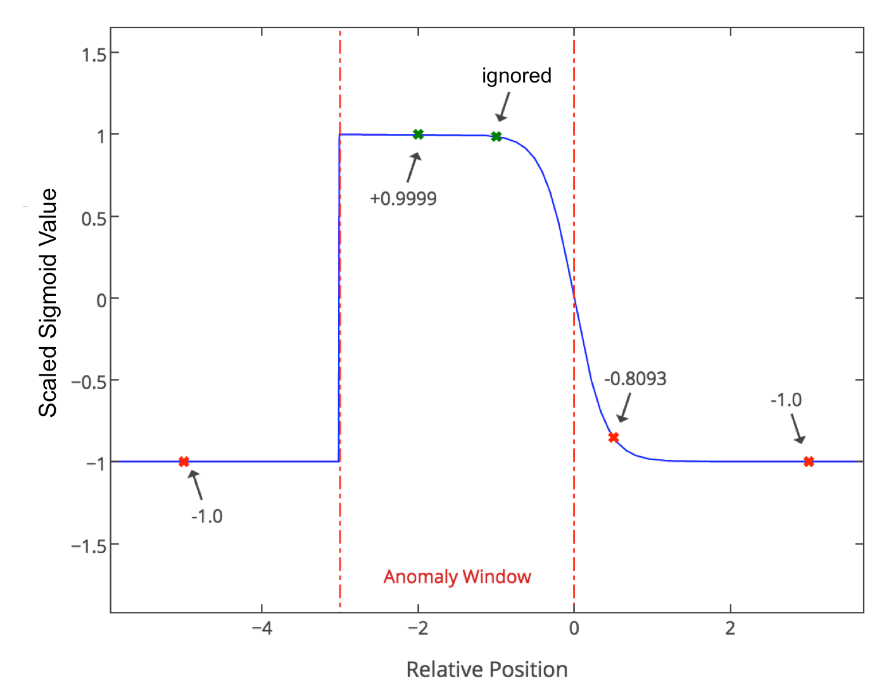
\includegraphics[width=\textwidth]{images/nabScoringExample.png}
    \caption{Scoring example for a sample anomaly window, where the values
represent the scaled sigmoid function. he first
point is an FP preceding the anomaly window (red dashed lines) and
contributes -1.0 to the score. Within the window we see two detections, and
only count the earliest TP for the score. There are two FPs after the window.
The first is less detrimental because it is close to the window, and the second
yields -1.0 because it’s too far after the window to be associated with the true
anomaly. TNs make no score contributions. The scaled sigmoid values are
multiplied by the relevant application profile weight. The NAB score for this example would calculate as: $-1.0A_{FP} + 0.9999A_{TP} - 0.8093A_{FP} - 1.0A_{FP} $}
    \label{nabSigmoidScoringFunction}
\end{figure}
To promote early detection NAB defines anomaly
windows. Each window represents a range of data points that is
centered around a ground truth anomaly label. Fig. 2 shows an
example using the data from Fig 1. A scoring function
(described in more detail below) uses these windows to
identify and weight true positives, false positives, and false
negatives. If there are multiple detections within a window, the
earliest detection is given credit and counted as a true positive.
Additional positive detections within the window are ignored.
The sigmoidal scoring function gives higher positive scores to
true positive detections earlier in a window and negative scores
to detections outside the window (i.e. the false positives).
These properties are illustrated in Fig. 3 with an example.
How large should the windows be? The earlier a detector
can reliably identify anomalies the better, implying these
windows should be as large as possible. The tradeoff with
extremely large windows is that random or unreliable
detections would be regularly reinforced. Using the underlying
assumption that true anomalies are rare, we define anomaly
window length to be 10\% the length of a data file, divided by
the number of anomalies in the given file. This technique
allows us to provide a generous window for early detections
and also allow the detector to get partial credit if detections are
soon after the ground truth anomaly. 10\% is a convenient
number but note the exact number is not critical. We tested a
range of window sizes (between 5\% and 20\%) and found that,
partly due to the scaled scoring function, the end score was not
sensitive to this percentage. Different applications may place different emphases as to
the relative importance of true positives vs. false negatives and
false positives. For example, the graph in Fig. 2 represents an
expensive industrial machine that one may find in a
manufacturing plant. A false negative leading to machine
failure in a factory can lead to production outages and be
extremely expensive. A false positive on the other hand might
require a technician to inspect the data more closely. As such
the cost of a false negative is far higher than the cost of a false
positive. Alternatively, an application monitoring the statuses
of individual servers in a datacenter might be sensitive to the
number of false positives and be fine with the occasional
missed anomaly since most server clusters are relatively fault
tolerant.To gauge how algorithms operate within these different
application scenarios, NAB introduces the notion of
application profiles. For TPs, FPs, FNs, and TNs, NAB applies
different relative weights associated with each profile to obtain
a separate score per profile. \\
\break
NAB includes three different application profiles: standard,
reward low FPs, and reward low FNs. The standard profile
assigns TPs, FPs, and FNs with relative weights (tied to the
window size) such that random detections made 10\% of the
time would get a zero final score on average. The latter two
profiles accredit greater penalties for FPs and FNs,
respectively. These two profiles are somewhat arbitrary but
designed to be illustrative of algorithm behavior. The NAB
codebase itself is designed such that the user can easily tweak
the relative weights and re-score all algorithms. The
application profiles thus help evaluate the sensitivity of
detectors to specific applications criteria.The combination of anomaly windows, a smooth temporal
scoring function (details in the next section), and the
introduction of application profiles allows researchers to
evaluate online anomaly detector implementations against the
requirements of the ideal detector. Specifically the overall
NAB scoring system evaluates real-time performance, prefers
earlier detection of anomalies, penalizes “spam” (i.e. FPs), and
provides realistic costs for the standard classification
evaluation metrics TP, FP, TN, and FN.\\
\break
Now to compute NAB score for an algorithm and a given application profile we use following procedure. Let $A$ be the application profile under consideration, with $A_{TP}$, $A_{FP}$	, $A_{FN}$ and $A_{TN}$ the corresponding weights for true positives, false positives, false negatives and true negatives.These weights are bounded $A_{TP} \geq 0$, $A_{TN} \leq 1$ and 
$A_{FP} \leq -1$, $A_{FN} \leq 0$. Let $D$ be the set
of data files and let $Y_d$ be the set of data instances detected as
anomalies for datafile d. (As discussed earlier, we remove
redundant detections: if an algorithm produces multiple
detections within the anomaly window, we retain only the
earliest one.) The number of windows with zero detections in
this data file is the number of false negatives, represented by $f_d$. The following scaled sigmoidal scoring function defines
the weight of individual detections given an anomaly window
and the relative position of each detection:
\begin{equation}
\sigma^{A}(y) = (A_{TP} - A_{FP})(\frac{1}{1+e^{5y}})-1
\label{sigmoidEquation}
\end{equation}
In equation (\ref{sigmoidEquation}), $y$ is the relative position of the detection within the
anomaly window. The parameters of the equation are set such that
the right end of the window evaluates to $\sigma(y = 0.0) = 0$ and it yields a max and min of $A_{TP}$ and $A_{FP}$, respectively. Every detection outside the window is counted as
a false positive and given a scaled negative score relative to the
preceding window. The function is designed such that
detections slightly after the window contribute less negative
scores than detections well after the window. Missing a
window completely is counted as a false negative and assigned
a score of $A_{FN}$. The raw score for a data file is the sum of the scores from
individual detections plus the impact of missing any windows:
\begin{equation}
S^A_d = (\sum_{y \in Y_d} \sigma^A(y)) + A_{FN}f_d
\label{weightsAccumulation}
\end{equation}
Equation (\ref{weightsAccumulation}), accumulates the weighted score for each true positive
and false positive, and detriments the total score with a
weighted count of all the false negatives. The benchmark raw score for a given algorithm is simply the sum of the raw scores
over all the data files in the corpus:
\begin{equation}
S^A = \sum_{d \in D} S^A_d
\label{allScore}
\end{equation}
The final reported score is a normalized NAB score computed as follows:
\begin{equation}
S^A_{NAB} = 100 \times \frac{S^A - S^A_{null}}{S^A_{perfect} - S^A_{null}}
\label{scoreNormalization}
\end{equation}
Here we scale the score based on the raw scores of a “perfect”
detector (one that outputs all true positives and no false
positives) and a “null” detector (one that outputs no anomaly
detections). It follows from equation (\ref{scoreNormalization}) that the maximum (normalized) score a detector can achieve on NAB is 100, and an algorithm making no detections will score 0.
\subsection{Comparing with others}
\begin{table}[H]
\centering
\begin{tabular}{llll}
 \hline  
\textbf{Algorithm} & low FN rate & low FP rate & Standard  \\
 \hline  
numenta   & 74.3202     & 63.1168 & 70.1011 \\
 \hline  
contextOSE          & 73.1817     & 66.9771 & 69.8996           \\
 \hline  
htmjava          & 70.4241     & 53.2569 & 65.5499        \\
\hline
numentaTM & 69.18506	& 56.6653	& 64.5534 \\
\hline
knncad & 64.8123 & 43.4085 & 57.9943\\
\hline
relativeEntropy & 58.8423 & 47.5984 & 54.6427\\
\hline
randomCutForest & 59.7488 & 38.3608 & 51.7171\\
\hline
twitterADVec & 53.5011 & 33.6101 & 47.062\\
\hline
predictionMultiStepLSTMMultiStep1Window50 & 59.3125 & 43.5927 & 43.2791\\
\hline
windowedGaussian & 47.41 & 20.868 & 39.6495\\
 \hline
predictionMultiStepLSTMMultiStep5Window20 & 41.6451 & 35.4072 & 39.1918\\
 \hline
predictionMultiStepLSTMMultiStep5Window20 & 40.8274 & 34.6116 & 38.3963\\
 \hline
predictionMultiStepLSTMMultiStep1Window200 & 40.2705 & 31.1383 & 36.0246\\
 \hline
skyline & 44.481 & 27.0812 & 35.687\\
 \hline
predictionMultiStepNNMultiStep4Window50 & 29.1037 & 25.6366 & 24.4352\\
 \hline
predictionMultiStepCNNMultiStep5Window30 & 21.228 & 19.6188 & 20.9474\\
 \hline
predictionMultiStepCNNMultiStep5Window20 & 21.5211 & 18.142 & 19.6384\\
 \hline
predictionMultiStepNNMultiStep5Window30 & 19.4988 & 18.0512 & 19.5921\\
 \hline
random & 27.201 & 5.76368 & 17.6554\\
 \hline
expose & 26.9209 & 3.19093 & 16.4367\\
 


  
\end{tabular}
\end{table}

\newpage
\section{Conclusion and Discussion}
\newpage
\section{Experiment Infrastructure}
\newpage
\subsection{Experiment Management using MLflow}
\newpage
\subsection{Parallel execution using Docker}
\newpage
\section{Best practices}
Following steps were taken to maximize the efficiency and speed of research:
\begin{enumerate}
	\item Use version control to track the code and share between different devices.
	\item Separate code from data. This will keep the code base small and easy to debug.
	\item Separate input data,working data and output data.
	\begin{itemize}
		\item \textbf{Input Data:} Input data-set that never change. For my case it is NAB and other external datasets.
		\item \textbf{Working Data:} nothing for now.
		\item \textbf{Output Data:} Results and threshold profiles in my case. 
	\end{itemize}
	\item Separate options from parameter. This is important:
 	\begin{itemize}
 		\item Options specify how your algorithm should run. For example data path, working directory and result directory path, epochs, learning rate and so on.
 		\item parameters are the result of training data. it includes the score and hyper-parameters. 
 	\end{itemize}
	
\end{enumerate}
\newpage
\subsection{Moving from jupyterlab to pycharm}
While working with jupyterlab notebook following routine was followed:
1- Load data with sample function
2- Write an algorithm
3- Test the results
4- Write general executeable .py file.
5- Get results on server

Since we needed to track change on two different places,
it was becoming harder to track the bugs and improve on efficiency.
That's why pycharm was selected to create executeable files and test
algorithms at the same time.
\section{Reference Usage}
\newpage
\section{References}
\begingroup
\nocite{*}
\renewcommand{\section}[2]{}
\bibliographystyle{IEEEtrans}`
\bibliography{third}
\endgroup
\end{document}
